\documentclass[tikz,border=2pt]{standalone}
% Preámbulo común de los diagramas TikZ (misma paleta y letra que las notas)
\usepackage[T1]{fontenc}\usepackage[utf8]{inputenc}
\usepackage{libertinus}\usepackage{libertinust1math}
\usepackage[defaultsans,scale=0.92]{lato}
\usepackage{amsmath,amssymb,bm}
\usepackage{tikz}\usetikzlibrary{calc,positioning,arrows.meta,shapes.geometric,decorations.pathreplacing,decorations.pathmorphing,fit,backgrounds}
\definecolor{snlazul}{HTML}{1E5AA8}\definecolor{snlnoche}{HTML}{14213D}\definecolor{snlvioleta}{HTML}{6C4AB6}
\definecolor{snlcoral}{HTML}{D1495B}\definecolor{snlambar}{HTML}{E09F3E}\definecolor{snlverde}{HTML}{2A9D8F}
\definecolor{snlteal}{HTML}{0F7173}\definecolor{snlgris}{HTML}{5C677D}\definecolor{snlfondo}{HTML}{F4F6FA}
\tikzset{>={Stealth[length=2.2mm]},
  bloque/.style={draw=#1,fill=#1!8,thick,rounded corners=2pt,minimum height=11mm,minimum width=20mm,align=center,font=\small},
  bloque/.default=snlazul,
  suma/.style={draw=snlnoche,thick,circle,inner sep=0pt,minimum size=5mm},
  flecha/.style={->,thick,draw=snlnoche},
  etq/.style={font=\small,text=snlnoche},
  nota/.style={font=\footnotesize\sffamily,text=snlgris,align=center}}

\begin{document}
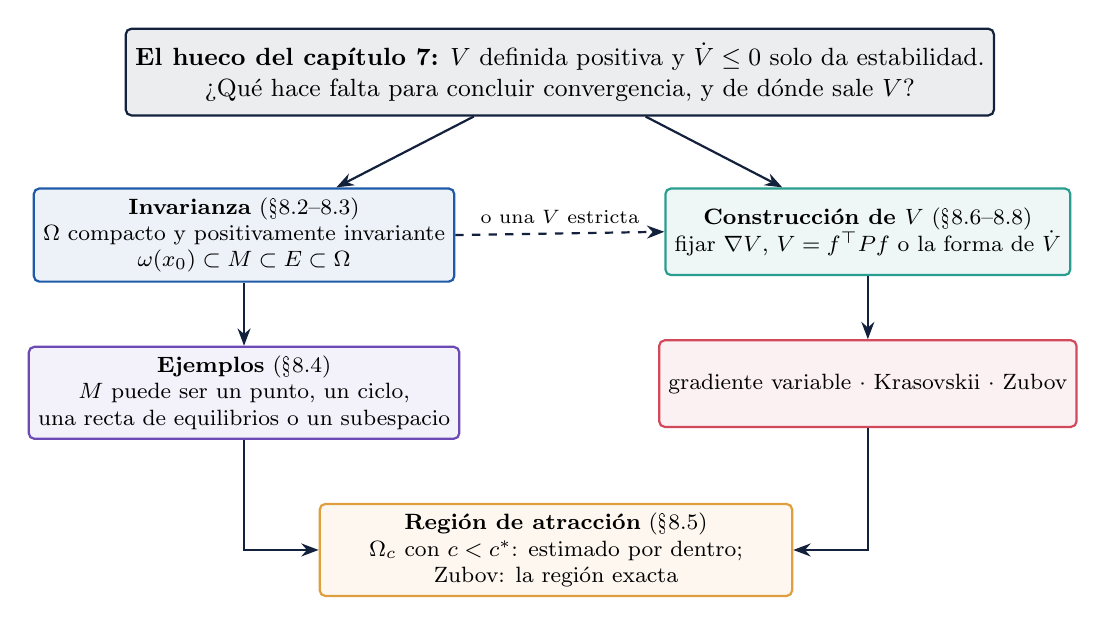
\begin{tikzpicture}[node distance=6mm and 8mm]
 \node[bloque=snlnoche,minimum width=104mm] (gap) {\textbf{El hueco del capítulo 7:} $V$ definida positiva y $\dot V\le0$ solo da estabilidad.\\ ¿Qué hace falta para concluir convergencia, y de dónde sale $V$?};
 \node[bloque=snlazul,below left=9mm and -42mm of gap,minimum width=50mm,font=\footnotesize] (inv) {\textbf{Invarianza} (\S8.2--8.3)\\ $\Omega$ compacto y positivamente invariante\\ $\omega(x_0)\subset M\subset E\subset\Omega$};
 \node[bloque=snlverde,below right=9mm and -42mm of gap,minimum width=50mm,font=\footnotesize] (cons) {\textbf{Construcción de $V$} (\S8.6--8.8)\\ fijar $\nabla V$, $V=f^{\top}Pf$ o la forma de $\dot V$};
 \node[bloque=snlvioleta,below=8mm of inv,minimum width=50mm,font=\footnotesize] (ej) {\textbf{Ejemplos} (\S8.4)\\ $M$ puede ser un punto, un ciclo,\\ una recta de equilibrios o un subespacio};
 \node[bloque=snlambar,below=8mm of $(ej.south)!0.5!(cons.south |- ej.south)$,minimum width=60mm,font=\footnotesize] (reg) {\textbf{Región de atracción} (\S8.5)\\ $\Omega_c$ con $c<c^*$: estimado por dentro;\\ Zubov: la región exacta};
 \node[bloque=snlcoral,below=8mm of cons,minimum width=50mm,font=\footnotesize] (met) {gradiente variable $\cdot$ Krasovskii $\cdot$ Zubov};
 \draw[flecha] (gap) -- (inv); \draw[flecha] (gap) -- (cons); \draw[flecha] (inv) -- (ej); \draw[flecha] (cons) -- (met);
 \draw[flecha] (ej) |- (reg); \draw[flecha] (met) |- (reg);
 \draw[flecha,dashed] (inv.east) -- node[above,font=\scriptsize]{o una $V$ estricta} (cons.west);
\end{tikzpicture}
\end{document}
